\documentclass[11pt,compress,t,notes=noshow, xcolor=table]{beamer}
\input{../../style/preamble_new}
\input{../../latex-math/basic-math.tex}
\input{../../latex-math/basic-ml.tex}

\title{Deep Learning for NLP II}

\begin{document}

\titlemeta{
Fine-Tuning Large Language Models
}{

}{
figure/finetuning
}{
\item BERT-style vs. SFT vs. prompting
\item Parameter-efficient fine-tuning
\item Adapter architectures
\item (Q)LoRA for efficient adaptation
\item Contrastive fine-tuning for embeddings
}

% ==============================================================================
% SECTION 1: Recap and Categorization
% ==============================================================================

\begin{frame}{Recall: Pre-Train / Fine-Tune Paradigm}

\vfill

\begin{itemize}
  \item \textbf{Pre-training:} Train a large model on massive unlabeled data
    \begin{itemize}
      \item Encoder-only (BERT): Masked Language Modeling (MLM)
      \item Decoder-only (GPT): Causal Language Modeling (CLM)
      \item Encoder-Decoder (T5): span corruption / seq2seq objectives
    \end{itemize}
  \item \textbf{Fine-tuning:} Adapt the pre-trained model to a downstream task
    \begin{itemize}
      \item The pre-trained weights serve as an initialization
      \item Much cheaper than training from scratch
      \item Even modest amounts of labeled data suffice
    \end{itemize}
  \item \ques But \textit{how} do we adapt/fine-tune? There is more than one answer!
\end{itemize}

\vfill

\end{frame}

% ------------------------------------------------------------------------------

\begin{frame}{A Taxonomy of Fine-Tuning Strategies}

\vfill

\textbf{Three major paradigms:}

\begin{enumerate}
  \item \textbf{BERT-style Fine-Tuning}\\
        Update \textit{all} model parameters; add a small task-specific head
  \item \textbf{Supervised Fine-Tuning (SFT) for Generative LLMs}\\
        Fine-tune a decoder on (instruction, response) pairs; no new head needed
  \item \textbf{Prompt-based Learning}\\
        Reformulate the task as a language modeling problem; minimal or \textit{no} gradient updates
\end{enumerate}

\vfill

\begin{center}
  These strategies differ in \textit{what} is updated, \textit{how} the task is represented, and \textit{how much} labeled data they need.
\end{center}

\vfill

\end{frame}

% ------------------------------------------------------------------------------

\begin{frame}{BERT-Style Fine-Tuning (1)}

\vfill

\textbf{Setup:}
\begin{itemize}
  \item Pre-trained encoder (BERT, RoBERTa, \ldots) with weights $\theta_0$
  \item Add a task-specific \textit{classification head} on top of \texttt{[CLS]} token
  \item Update \textbf{all} parameters $\theta$ jointly on labeled data
\end{itemize}

\vfill

\textbf{Objective (classification):}
$$\mathcal{L} = -\sum_{(x,y) \in \mathcal{D}} \log p_\theta(y \mid x)$$

\vfill

\textbf{Key properties:}
\begin{itemize}
  \item One separate model per task (different fine-tuned copies)
  \item Strong performance on many NLU benchmarks,\\e.g., \citebutton{GLUE (Wang et al., 2019a)}{https://gluebenchmark.com/} \citebutton{SuperGLUE (Wang et al., 2019b)}{https://super.gluebenchmark.com/}
  \item Requires labeled data; \textbf{not} a generative approach
\end{itemize}

\vfill

\end{frame}

% ------------------------------------------------------------------------------

\begin{frame}{BERT-Style Fine-Tuning (2)}

\vfill

\textbf{Supported task types:}

\begin{itemize}
  \item \textbf{Sequence classification:} Pool \texttt{[CLS]} $\to$ linear layer $\to$ softmax\\
        Examples: sentiment analysis, NLI, document classification
  \item \textbf{Token classification:} Use each token's representation $\to$ per-token linear; Examples: NER, POS tagging, chunking
  \item \textbf{Span extraction / QA:} Predict start \& end positions\\
        Example: SQuAD reading comprehension
\end{itemize}

\vfill

\textbf{Practical hyperparameters: \citebutton{Devlin et al., 2019}{https://aclanthology.org/N19-1423/}}
\begin{itemize}
  \item Adam lr: $2\text{e-5}$, $3\text{e-5}$, $5\text{e-5}$; Batch size: 16, 32; Epochs: 2--4
\end{itemize}

\vfill

\end{frame}

% ------------------------------------------------------------------------------

\begin{frame}{Fine-Tuning BERT}
	\begin{figure}
	\centering
		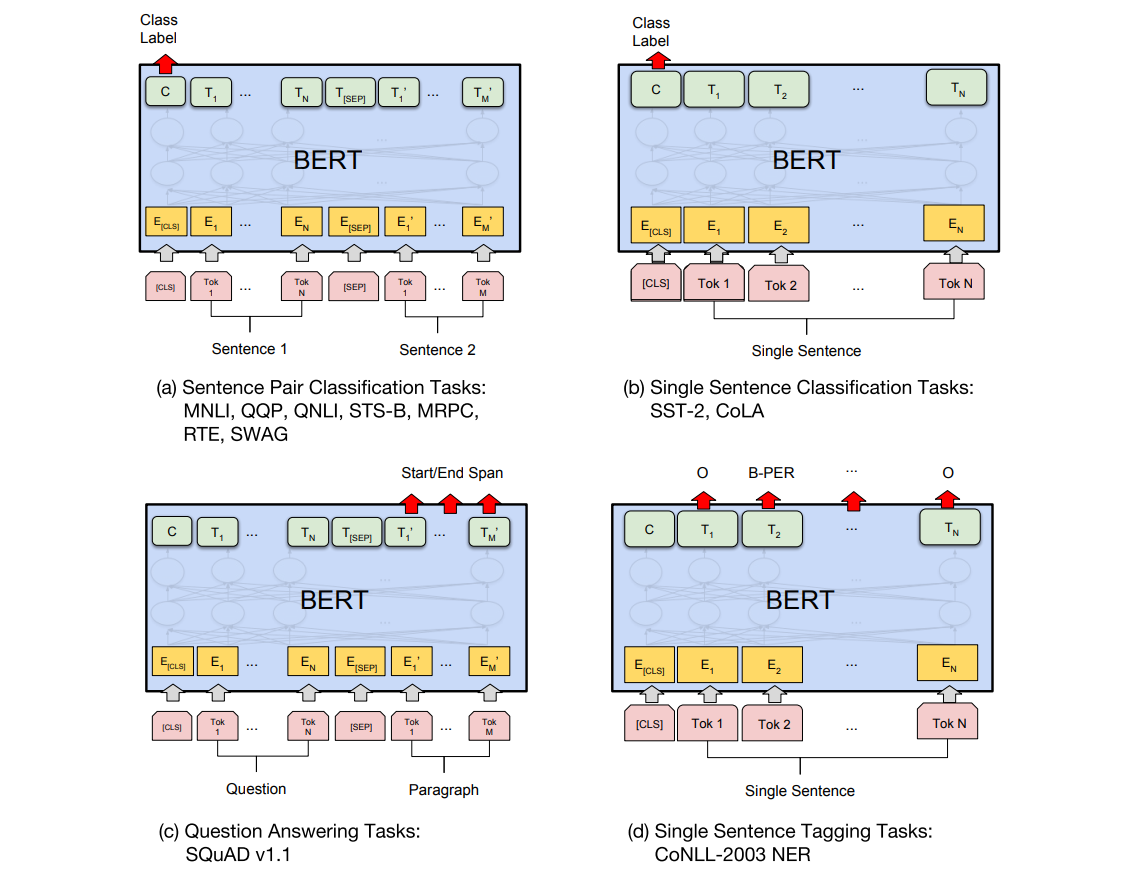
\includegraphics[width = 10cm]{figure/bert-finetune.png}\\ 
	\citebutton{Source: Devlin et al., 2019}{https://aclanthology.org/N19-1423.pdf}
	\end{figure}
\end{frame}

% ------------------------------------------------------------------------------

\begin{frame}{Supervised Fine-Tuning (SFT) for Generative LLMs}

\vfill

\textbf{Generative LLMs} (GPT-2/3/4, LLaMA, Mistral, \ldots):
\begin{itemize}
  \item \textbf{Architecture:} Decoder-only Transformer
  \item \textbf{Pre-training:} Autoregressive LM $\to$ predict next token
  \item \textbf{No separate classification head} -- output is free-form text
\end{itemize}

\vfill

\textbf{SFT:} Fine-tune on curated (instruction, response) pairs
$$\mathcal{L}_\text{SFT} = -\sum_{t} \log p_\theta(y_t \mid x, y_{<t})$$

\begin{itemize}
  \item Teach the model to \textit{follow instructions}
  \item Examples: summarize, translate, answer questions, write code
  \item Foundation for RLHF / DPO alignment pipelines
\end{itemize}

\vfill

\end{frame}

% ------------------------------------------------------------------------------

\begin{frame}{Prompt-Based Learning}

\vfill

\textbf{Core idea:} Reformulate the task so it \textit{looks like} the pre-training objective

\begin{itemize}
  \item \textbf{Zero-shot prompting:}\\
        ``\texttt{Classify the sentiment of: [text]. Answer positive or negative.}''
  \item[] $\to$ No gradient update; relies entirely on pre-trained knowledge
  \item \textbf{Few-shot (in-context) learning:}\\
        Prepend a few labeled examples to the prompt; still no training
  \item \textbf{Prompt tuning / prefix tuning:}\\
        Learn a small set of soft (continuous) prompt tokens; freeze the LLM
        \citebutton{Lester et al., 2021}{https://aclanthology.org/2021.emnlp-main.243/}
        \citebutton{Li \& Liang, 2021}{https://arxiv.org/abs/2101.00190}
\end{itemize}

\vfill

\textbf{Key benefit:} One shared model for all tasks; no task-specific copies

\vfill

\end{frame}

% ------------------------------------------------------------------------------

\begin{frame}{Prompt-Tuning}
	\begin{figure}
	\centering
		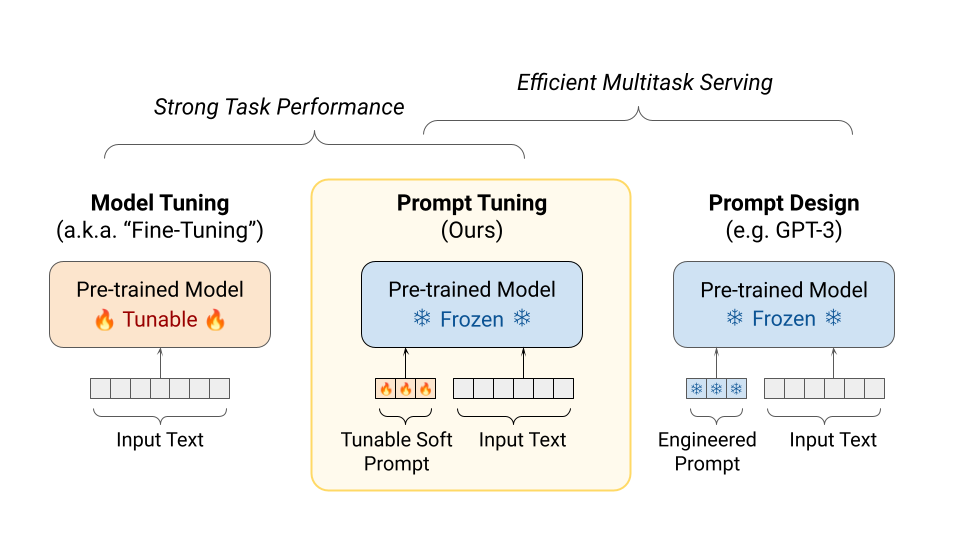
\includegraphics[width = 11cm]{figure/prompttuning.png}\\ 
	\citebutton{Source: Lester et al., 2021}{https://aclanthology.org/2021.emnlp-main.243/}
	\end{figure}
\end{frame}

% ------------------------------------------------------------------------------

\begin{frame}{Comparison: FT vs. SFT vs. Prompt-based}

\vfill
{\scriptsize
\renewcommand{\arraystretch}{1.5}
\begin{tabular}{lccc}
\hline
\textbf{Property} & \textbf{BERT Fine-Tune} & \textbf{SFT (Gen. LLM)} & \textbf{Prompt-Based} \\
\hline
Architecture & Encoder & Decoder & Both \\
Updated params & All $|\theta|$ & All $|\theta|$ & Few / None \\
Task representation & Classification head & Free text & In-context / soft prompt \\
Labeled data needed & Many & Moderate & Few / None \\
One model per task? & Yes & Often & No \\
Generative? & No & Yes & Yes \\
\hline
\end{tabular}
}
\vfill

\ques Why does updating \textit{all} parameters become a problem at scale?

\vfill

\end{frame}

% ------------------------------------------------------------------------------

\begin{frame}{Problem: Full Fine-Tuning at Scale}

\vfill

\begin{itemize}
  \item GPT-3: $|\theta| = 175\text{B}$ parameters
  \item Storing one fine-tuned copy requires $\approx$ 350 GB (fp16)
  \item Deploying $k$ tasks $\Rightarrow$ $k \times 350$ GB storage
  \item Training requires optimizer states: \\
	$\to$ Adam requires $\sim 3\times$ model size in memory
\end{itemize}

\vfill

\textbf{Consequence:} Full fine-tuning of very large models is
\begin{itemize}
  \item Prohibitively \textit{expensive} (compute, memory, storage)
  \item Prone to \textit{catastrophic forgetting} of pre-trained knowledge
  \item Inefficient when deployed \textit{across many tasks}
\end{itemize}

\vfill

$\to$ \textbf{Parameter-Efficient Fine-Tuning (PEFT)} methods address this!

\vfill

\end{frame}

% ==============================================================================
% SECTION 2: Adapters
% ==============================================================================

\begin{frame}{PEFT: Overview}

\vfill

\textbf{Goal:} Adapt a large pre-trained model to downstream tasks while updating only a \textit{small fraction} of parameters

\vfill

\textbf{Main families:}
\begin{itemize}
  \item \textbf{Adapter layers} -- insert small bottleneck modules \textit{inside} each Transformer block \citebutton{Houlsby et al., 2019}{https://proceedings.mlr.press/v97/houlsby19a}
  \item \textbf{Prefix / Prompt Tuning} -- prepend learnable tokens to the sequence \citebutton{Lester et al., 2021}{https://aclanthology.org/2021.emnlp-main.243/}
  \item \textbf{Low-rank decomposition (LoRA)} -- approximate weight updates with low-rank matrices \citebutton{Hu et al., 2022}{https://arxiv.org/abs/2106.09685}
  \item \textbf{Selective / sparse updates} -- update only a subset of existing parameters (e.g., BitFit)
\end{itemize}

\vfill

\end{frame}

% ------------------------------------------------------------------------------

\begin{frame}{Adapter Layers: Core Idea}

\vfill

\textbf{Proposed by Houlsby et al. (2019):}
\begin{itemize}
  \item Insert small \textit{adapter modules} after each sub-layer of the Transformer
  \item The pre-trained weights are \textbf{frozen}; only adapters are trained
  \item Each adapter is a \textit{bottleneck} network:
\end{itemize}

\vfill

\textbf{Adapter architecture:}
$$\text{Adapter}(h) = h + W_\text{up} \cdot \sigma(W_\text{down} \cdot h)$$
\begin{itemize}
  \item $h \in \mathbb{R}^d$: hidden state from Transformer layer
  \item $W_\text{down} \in \mathbb{R}^{m \times d}$, $W_\text{up} \in \mathbb{R}^{d \times m}$, with $m \ll d$ (bottleneck)
  \item Residual connection ensures stability at initialization ($W_\text{up} W_\text{down} \approx 0$)
\end{itemize}

\vfill

\end{frame}

% ------------------------------------------------------------------------------

\begin{frame}{Adapter Layers: Placement}

\vfill

\begin{columns}[T]
\begin{column}{0.55\textwidth}
\textbf{Placement in the Transformer block:}
\begin{itemize}
  \item After each \textbf{MHA} sub-layer
  \item After each \textbf{FF} sub-layer
  \item Each followed by layer norm
  \item Two modules per Transformer layer
\end{itemize}

\vfill

\textbf{BERT-base:} ($d = 768$, $L = 12$):
\begin{itemize}
  \item $m = 64$: $\approx$ 0.5M trainable params
  \item $m = 256$: $\approx$ 3.6M trainable params
  \item vs.\ $\approx$ 110M total (BERT-base)
\end{itemize}
\end{column}
\begin{column}{0.4\textwidth}
\vspace{1.7cm}
\begin{center}
\begin{tabular}{|c|}
\hline
\textbf{Layer Norm} \\
\hline
Feed-Forward \\
\hline
\cellcolor{blue!20}\textbf{Adapter} \\
\hline
\textbf{Layer Norm} \\
\hline
Multi-Head Attn \\
\hline
\cellcolor{blue!20}\textbf{Adapter} \\
\hline
\end{tabular}
\end{center}
\end{column}
\end{columns}

\vfill

\end{frame}

% ------------------------------------------------------------------------------

\begin{frame}{Adapter Layers: Key Properties}

\vfill

\textbf{Advantages:}
\begin{itemize}
  \item \textbf{Parameter efficiency:} $< 1\%$ additional parameters per task
  \item \textbf{Shared backbone:} One pre-trained model; swap only small adapters
  \item \textbf{No catastrophic forgetting:} Frozen backbone preserves pre-trained knowledge
  \item \textbf{Modularity:} Adapters for different tasks / languages can be combined
\end{itemize}

\vfill

\textbf{Limitation:}
\begin{itemize}
  \item Adapters are processed \textit{sequentially} $\Rightarrow$ added inference latency
  \item In online inference (batch size = 1), latency increase can be $> 20\%$ \citebutton{Hu et al., 2022}{https://arxiv.org/abs/2106.09685}
  \item Harder to exploit hardware parallelism (vs.\ frozen weights merged at inference time)
\end{itemize}

\vfill

\end{frame}

% ------------------------------------------------------------------------------

\begin{frame}{AdapterHub}

\vfill

\textbf{Problem:} Sharing and re-using trained adapters is not straightforward

\vfill

\citebutton{Pfeiffer et al. (2020)}{https://aclanthology.org/2020.emnlp-demos.7/} propose \textbf{AdapterHub}:
\begin{itemize}
  \item A \textit{repository} for pre-trained adapters (analogous to HuggingFace)
  \item Dynamic ``stitching-in'' of adapters into any compatible backbone
  \item Built on top of HuggingFace \texttt{transformers}; minimal code changes required
  \item Supports BERT, RoBERTa, XLM-R and more
\end{itemize}

\vfill

\textbf{Workflow:}
\begin{enumerate}
  \item Download pre-trained backbone
  \item Load adapter weights from \texttt{AdapterHub.ml}
  \item Train only the adapter; share back to the hub
\end{enumerate}

\vfill

\end{frame}

% ------------------------------------------------------------------------------

\begin{frame}{AdapterFusion}

\vfill

\textbf{Motivation:} Can we \textit{combine} adapters trained on different tasks without retraining?

\vfill

\textbf{Sequential fine-tuning} and \textbf{multi-task learning} both suffer from:
\begin{itemize}
  \item Catastrophic forgetting (sequential)
  \item Dataset balancing difficulties (multi-task)
\end{itemize}

\vfill

\textbf{AdapterFusion} \citebutton{Pfeiffer et al. (2021)}{https://aclanthology.org/2021.eacl-main.39/} propose a \textit{two-stage} learning algorithm:
\begin{enumerate}
  \item \textbf{Knowledge extraction:} Train $N$ task-specific adapters independently (frozen backbone)
  \item \textbf{Knowledge composition:} Learn a \textit{fusion layer} that attends over the adapters
\end{enumerate}

\vfill

\end{frame}

% ------------------------------------------------------------------------------

\begin{frame}{AdapterFusion: The Fusion Layer}

\vfill

\textbf{Fusion mechanism} (attention over adapter outputs):

At each adapter position, given hidden state $h$ and adapter outputs $Z = [z_1, \ldots, z_N]$:
$$\text{AdapterFusion}(h, Z) = \text{softmax}\!\left(\frac{(hW_Q)(ZW_K)^\top}{\sqrt{d}}\right) (ZW_V)$$

\begin{itemize}
  \item $W_Q, W_K, W_V$: small learnable projection matrices
  \item The backbone and individual adapters remain \textbf{frozen}
  \item Only the fusion layer parameters are updated in stage 2
\end{itemize}

\vfill

\textbf{Result:} Non-destructive task composition -- evaluated on 16 diverse NLU tasks, outperforms full fine-tuning and multi-task learning

\vfill

\end{frame}

% ==============================================================================
% SECTION 3: LoRA / QLoRA
% ==============================================================================

\begin{frame}{LoRA: Motivation}

\vfill

\textbf{Key observation} \citebutton{Aghajanyan et al., 2020}{https://arxiv.org/abs/2012.13255}:
\begin{itemize}
  \item Pre-trained language models have a low \textit{intrinsic dimension}
  \item They can learn effectively even when projected into a smaller subspace
\end{itemize}

\vfill

\textbf{LoRA hypothesis} \citebutton{Hu et al., ICLR 2022}{https://arxiv.org/abs/2106.09685}:
\begin{itemize}
  \item The \textit{weight updates} $\Delta W$ during adaptation also have low intrinsic rank
  \item We can represent $\Delta W \approx BA$ where $B \in \mathbb{R}^{d \times r}$, $A \in \mathbb{R}^{r \times k}$, $r \ll \min(d, k)$
\end{itemize}

\vfill

\textbf{Consequence:} Instead of updating the full weight matrix, train only the low-rank decomposition $B$ and $A$ -- much fewer parameters!

\vfill

\end{frame}

% ------------------------------------------------------------------------------

\begin{frame}{LoRA: Low-Rank Adaptation of Large Language Models}

\vfill

\textbf{Modified forward pass:}

For a pre-trained weight matrix $W_0 \in \mathbb{R}^{d \times k}$:

$$h = W_0 x + \Delta W x = W_0 x + B A x$$

\begin{itemize}
  \item $W_0$ is \textbf{frozen} -- no gradient flows through it
  \item $B \in \mathbb{R}^{d \times r}$, $A \in \mathbb{R}^{r \times k}$ are \textbf{trainable}
  \item Rank $r \ll \min(d, k)$ (e.g., $r = 4$ or $r = 8$)
\end{itemize}

\vfill

\textbf{Initialization:}
\begin{itemize}
  \item $A \sim \mathcal{N}(0, \sigma^2)$ (random Gaussian)
  \item $B = 0$ $\Rightarrow$ $\Delta W = BA = 0$ at the start of training
  \item Scaled by $\frac{\alpha}{r}$ (where $\alpha$ is a fixed constant)
\end{itemize}

\vfill

\end{frame}

% ------------------------------------------------------------------------------

\begin{frame}{LoRA: Parameter Savings}

\vfill

\textbf{Example: GPT-3 175B, applying LoRA to $W_q$ and $W_v$ ($d = 12.288$)}

\begin{itemize}
  \item Full fine-tuning: $|\Delta\theta| = |\theta_0| = 175$B parameters
  \item LoRA with $r = 4$: $|\Theta| = 2 \times 2 \times d \times r = 4 \times 12288 \times 4 \approx 200\text{k}$ per layer
\end{itemize}

\vfill

\textbf{Reduction: $\approx 10{,}000\times$ fewer trainable parameters!}

\vfill

\textbf{Memory savings:}
\begin{itemize}
  \item No optimizer states needed for $W_0$ (frozen)
  \item Adam: $3\times$ less GPU memory vs.\ full fine-tuning
  \item No gradient computation through $W_0$
\end{itemize}

\vfill

\end{frame}

% ------------------------------------------------------------------------------

\begin{frame}{LoRA: No Inference Latency}

\vfill

\textbf{Key advantage over adapters:}

\begin{itemize}
  \item After training, we can \textit{merge} the LoRA weights back into the backbone:
  $$W = W_0 + BA$$
  \item The merged weight $W$ has the \textit{same shape} as $W_0$
  \item \textbf{Zero additional inference latency} -- the merged model runs identically to the original
\end{itemize}

\vfill

\textbf{Task switching:}
\begin{itemize}
  \item Recover $W_0$ by subtracting: $W_0 = W - BA$
  \item Load a different $B'A'$ for a different task
  \item Very low memory overhead for switching
\end{itemize}

\vfill

\end{frame}

% ------------------------------------------------------------------------------

\begin{frame}{LoRA: Where to Apply?}

\vfill

\textbf{Transformer weight matrices:}
\begin{itemize}
  \item Self-attention: $W_q, W_k, W_v, W_o$
  \item Feed-forward: $W_1, W_2$
\end{itemize}

\vfill

\textbf{Empirical findings (Hu et al., 2022):}
\begin{itemize}
  \item Adapting $W_q$ and $W_v$ alone gives strong results
  \item Spreading rank across more weight matrices (lower $r$ each) outperforms concentrating rank in one matrix
  \item Rank $r = 4$ or $r = 8$ typically sufficient; increasing beyond $r = 64$ gives diminishing returns
\end{itemize}

\vfill

\textbf{LoRA is orthogonal to many methods} -- can be combined with prefix tuning, quantization, etc.

\vfill

\end{frame}

% ------------------------------------------------------------------------------

\begin{frame}{LoRA: Experimental Results}

\vfill

\textbf{RoBERTa, DeBERTa (NLU):}
\begin{itemize}
  \item LoRA matches or exceeds full fine-tuning on GLUE benchmarks
  \item Only $\approx 0.3\%$ of parameters updated (vs.\ 100\% for full fine-tuning)
\end{itemize}

\vfill

\textbf{GPT-2 (NLG -- E2E, WebNLG, DART):}
\begin{itemize}
  \item LoRA outperforms adapter-based methods and prefix tuning
  \item Training throughput $\approx 25\%$ higher than full fine-tuning
\end{itemize}

\vfill

\textbf{GPT-3 175B:}
\begin{itemize}
  \item LoRA with $r = 4$ matches full fine-tuning on WikiSQL and SAMSum
  \item Full fine-tuning of GPT-3 requires $\approx 1.2$TB of GPU memory; LoRA: $\approx 350$ GB
\end{itemize}

\vfill

\end{frame}

% ------------------------------------------------------------------------------

\begin{frame}{QLoRA: Efficient Fine-Tuning of Quantized LLMs}

\vfill

\textbf{Challenge:} Even with LoRA, fine-tuning a 65B parameter model requires $> 780$ GB GPU memory (fp16)

\vfill

\textbf{QLoRA} \citebutton{Dettmers et al., 2023}{https://arxiv.org/abs/2305.14314} combines:
\begin{enumerate}
  \item \textbf{4-bit quantization} of the pre-trained model (backbone frozen at 4-bit)
  \item \textbf{LoRA adapters} trained in bf16/fp16 on top of the quantized backbone
  \item Gradients are backpropagated \textit{through} the quantized backbone into the LoRA parameters
\end{enumerate}

\vfill

\textbf{Result:} Fine-tune a 65B model on a \textit{single 48 GB GPU}

\vfill

\end{frame}

% ------------------------------------------------------------------------------

\begin{frame}{QLoRA: Key Innovations}

\vfill

\textbf{(a) 4-bit NormalFloat (NF4):}
\begin{itemize}
  \item New data type, information-theoretically optimal for normally distributed weights
  \item Outperforms standard 4-bit integers and 4-bit floats empirically
\end{itemize}

\vfill

\textbf{(b) Double Quantization:}
\begin{itemize}
  \item Quantize the quantization constants themselves (second level of compression)
  \item Saves $\approx$ 0.37 bits per parameter ($\approx$ 3 GB for a 65B model)
\end{itemize}

\vfill

\textbf{(c) Paged Optimizers:}
\begin{itemize}
  \item Use NVIDIA unified memory to handle gradient checkpointing spikes
  \item Avoids out-of-memory errors when processing long sequences
\end{itemize}

\vfill

\end{frame}

% ------------------------------------------------------------------------------

\begin{frame}{QLoRA: Results -- The Guanaco Models}

\vfill

\textbf{Guanaco family:} 65B, 33B, 13B, 7B parameter models fine-tuned with QLoRA on OASST1 (9k samples)

\vfill

\begin{tabular}{lcc}
\hline
\textbf{Model} & \textbf{GPU mem.} & \textbf{Elo (Vicuna bench.)} \\
\hline
GPT-4 & -- & 1348 \\
\rowcolor{blue!10}
Guanaco 65B & 41 GB & 1022 \\
Guanaco 33B & 21 GB & 992 \\
ChatGPT & -- & 966 \\
Guanaco 13B & 10 GB & 916 \\
\hline
\end{tabular}

\vfill

\begin{itemize}
  \item Guanaco 65B reaches \textbf{99.3\%} of ChatGPT performance\\ (Vicuna benchmark)
  \item Trained in \textbf{24 hours} on a single GPU
  \item Data quality $\gg$ data size: 9k high-quality samples beat\\ 450k FLAN samples
\end{itemize}

\vfill

\end{frame}

% ------------------------------------------------------------------------------

\begin{frame}{LoRA vs.\ QLoRA: Summary}

\vfill

\renewcommand{\arraystretch}{1.4}
\begin{tabular}{lcc}
\hline
\textbf{Property} & \textbf{LoRA} & \textbf{QLoRA} \\
\hline
Backbone precision & fp16/bf16 & \textbf{4-bit NF4} \\
LoRA adapter precision & fp16/bf16 & fp16/bf16 \\
Memory saving vs.\ full FT & $\approx 3\times$ & $\approx 16\times$ \\
Inference latency & None (merge) & None (dequant + merge) \\
Performance vs.\ full FT & On-par & On-par \\
65B model GPU req. & $\sim$350 GB & \textbf{$< 48$ GB} \\
\hline
\end{tabular}

\vfill

\textbf{Bottom line:} QLoRA makes fine-tuning frontier-scale models accessible on consumer hardware

\vfill

\end{frame}

% ==============================================================================
% SECTION 4: Contrastive Fine-Tuning of Embedding Models
% ==============================================================================

\begin{frame}{From Classification to Embeddings}

\vfill

\textbf{Recap: BERT for classification}
\begin{itemize}
  \item Fine-tune with a cross-entropy classification head
  \item Optimizes \textit{correct label prediction}, not embedding geometry
  \item The resulting embeddings are not necessarily good for retrieval / similarity
\end{itemize}

\vfill

\textbf{Other use cases requiring embeddings:}
\begin{itemize}
  \item Semantic textual similarity (STS)
  \item Dense retrieval / RAG (query $\leftrightarrow$ document matching)
  \item Clustering, deduplication, semantic search
\end{itemize}

\vfill

\ques How do we fine-tune LLMs to produce \textit{useful} sentence / document embeddings?

\vfill

\end{frame}

% ------------------------------------------------------------------------------

\begin{frame}{Contrastive Learning: Core Idea}

\vfill

\textbf{Goal:} Shape the embedding space so that: 
\begin{itemize}
  \item \textbf{Similar} sentences $\to$ \textbf{close} in embedding space
  \item \textbf{Dissimilar} sentences $\to$ \textbf{far apart} in embedding space
\end{itemize}

\vspace{1em}

\textbf{Triplet formulation:}
\begin{itemize}
  \item \textbf{Anchor} $a$: the query / reference sentence
  \item \textbf{Positive} $p$: a semantically similar sentence
  \item \textbf{Negative} $n$: a semantically dissimilar sentence
\end{itemize}

\vfill

\textbf{Triplet loss:}
$$\mathcal{L}_\text{triplet} = \max\!\left(0,\; d(a, p) - d(a, n) + \epsilon\right)$$
where $d(\cdot, \cdot)$ is a distance metric (e.g., $1 - \cos(\cdot, \cdot)$) and $\epsilon > 0$ is a margin

\vfill

\end{frame}

% ------------------------------------------------------------------------------

\begin{frame}{Sentence-BERT (SBERT)}

\vfill

\textbf{SBERT} \citebutton{Reimers \& Gurevych (2019)}{https://aclanthology.org/D19-1410/}:

\begin{itemize}
  \item Fine-tune BERT with \textit{siamese} and \textit{triplet} network architectures
  \item \textbf{Siamese:} Two identical BERT encoders sharing weights; compare pooled representations
  \item \textbf{Objective:} Mean-pooled \texttt{[CLS]} output; trained on NLI and STS data
\end{itemize}

\vfill

\textbf{Training objectives used in SBERT:}
\begin{enumerate}
  \item \textbf{Classification (NLI):} Concatenate $[u; v; |u - v|]$; softmax over entailment/neutral/contradiction
  \item \textbf{Regression (STS):} Cosine similarity of $u$ and $v$; MSE loss against gold similarity score
  \item \textbf{Triplet objective:} Directly minimize triplet loss
\end{enumerate}

\vfill

\end{frame}

% ------------------------------------------------------------------------------

\begin{frame}{SimCSE: Simple Contrastive Learning of Sentence Embeddings}

\vfill

\textbf{SimCSE} \citebutton{Gao et al. (2021)}{https://aclanthology.org/2021.emnlp-main.552/} uses \textit{dropout} as minimal data augmentation

\vfill

\textbf{Unsupervised SimCSE:}
\begin{itemize}
  \item Pass the same sentence through the encoder \textit{twice} with different dropout masks
  \item The two resulting embeddings form a \textbf{positive pair}
  \item All other sentences in the batch serve as \textbf{in-batch negatives}
\end{itemize}

\vfill

\textbf{In-batch negative loss:}
$$\mathcal{L} = -\log \frac{e^{\text{sim}(h_i, h_i^+)/\tau}}{\sum_{j=1}^{N} e^{\text{sim}(h_i, h_j^+)/\tau}}$$
where $\tau$ is temperature and $h_i^+$ is the augmented positive for anchor $h_i$

\vfill

\end{frame}

% ------------------------------------------------------------------------------

\begin{frame}{SimCSE: Supervised and Hard Negatives}

\vfill

\textbf{Supervised SimCSE:}
\begin{itemize}
  \item Use NLI data: premise as anchor, \textit{entailment} as positive, \textit{contradiction} as hard negative
  \item Objective includes hard negatives $h_i^-$:
\end{itemize}

$$\mathcal{L} = -\log \frac{e^{\text{sim}(h_i, h_i^+)/\tau}}{\sum_{j=1}^{N} \left(e^{\text{sim}(h_i, h_j^+)/\tau} + e^{\text{sim}(h_i, h_j^-)/\tau}\right)}$$

\vfill

\textbf{Why hard negatives matter:}
\begin{itemize}
  \item Random negatives are easy -- the model learns little from them
  \item Hard negatives are superficially similar but semantically different
  \item Forcing the model to separate them sharpens the embedding space
\end{itemize}

\vfill

\end{frame}

% ------------------------------------------------------------------------------

\begin{frame}{Contrastive Fine-Tuning: Dense Retrieval}

\vfill

\textbf{Dense Passage Retrieval (DPR)} \citebutton{Karpukhin et al. (2020)}{https://aclanthology.org/2020.emnlp-main.550/}:
\begin{itemize}
  \item Two separate BERT encoders: one for \textit{queries}, one for \textit{passages}
  \item Fine-tuned with in-batch negatives + hard negatives from BM25
  \item Positive pairs: (question, gold answer paragraph) from QA datasets
\end{itemize}

\vfill

\textbf{Modern recipe for embedding model fine-tuning:}
\begin{enumerate}
  \item Start from a strong pre-trained LLM or BERT variant
  \item Mine (hard) negative pairs -- e.g., using BM25 or a teacher model
  \item Train with contrastive loss + in-batch negatives
  \item Scale up: large batches, multi-GPU, GradCache for memory efficiency
\end{enumerate}

\vfill

\end{frame}

% ------------------------------------------------------------------------------

\begin{frame}{Modern Embedding Models: E5, GTE, BGE}

\vfill

\textbf{Commonalities of recent embedding models:}
\begin{itemize}
  \item Large LLM backbone (e.g., LLaMA, Mistral, or Qwen)
  \item Multi-stage training:\\ Weak Supervision $\to$ Supervised contrastive fine-tuning
  \item Massive mined datasets \textit{with hard negatives}
\end{itemize}

\vfill

\textbf{Examples:}
\begin{itemize}
	\item \textbf{E5} \citebutton{Wang et al., 2022}{https://arxiv.org/abs/2212.03533}: Contrastive pre-training on CCPairs then SFT
	\item \textbf{BGE} \citebutton{Xiao et al., 2023}{https://arxiv.org/abs/2309.07597}: RetroMAE + contrastive SFT; instruction-enhanced
	\item \textbf{GTE} \citebutton{Li et al., 2023}{https://arxiv.org/abs/2308.03281}: Multi-stage contrastive training pipeline
\end{itemize}

\vfill

\textbf{Key insight:} Scale of contrastive data $>$ scale of backbone parameters for retrieval tasks

\vfill

\end{frame}

% ------------------------------------------------------------------------------

\begin{frame}{Contrastive Fine-Tuning: Anisotropy Problem}

\vfill

\textbf{Problem: representation degeneration} \citebutton{Gao et al. (2019)}{https://openreview.net/forum?id=SkEYojRqtm}

\begin{itemize}
  \item BERT sentence embeddings (without contrastive training) cluster in a narrow cone
  \item High cosine similarity between semantically unrelated sentences
  \item The embedding space is \textit{anisotropic}: most variance in one direction
\end{itemize}

\vfill

\textbf{Contrastive training fixes this:}
\begin{itemize}
  \item Pushes embeddings apart $\Rightarrow$ more uniform distribution on the hypersphere
  \item SimCSE measures this via \textit{alignment} (positive pairs close) and \textit{uniformity} (all points spread)
\end{itemize}

$$\mathcal{L}_\text{uniform} = \log \mathbb{E}_{x, y \sim p_\text{data}}\left[e^{-2\|f(x) - f(y)\|^2}\right]$$

\vfill

\end{frame}

% ------------------------------------------------------------------------------

\begin{frame}{Contrastive Fine-Tuning: Practical Considerations}

\vfill

\textbf{Negative mining strategies:}
\begin{itemize}
  \item \textbf{Random in-batch negatives:} Simple, effective at large batch sizes
  \item \textbf{BM25 hard negatives:} Lexically similar but semantically different documents
  \item \textbf{Cross-encoder reranking:} Use a stronger model to score and mine hard negatives
  \item \textbf{Self-mined negatives:} Use the embedding model itself to find near-misses
\end{itemize}

\vfill

\textbf{Pooling strategies:}
\begin{itemize}
  \item \textbf{CLS pooling:} Use the \texttt{[CLS]} token representation
  \item \textbf{Mean pooling:} Average all token representations (often better)
  \item \textbf{Last token:} Common for decoder-only LLMs (EOS token)
\end{itemize}

\vfill

\end{frame}

% ==============================================================================
% SECTION 5: Summary
% ==============================================================================

\begin{frame}{Summary: Overview on strategies}

\vfill

{\footnotesize
\renewcommand{\arraystretch}{1.4}
\begin{tabular}{lcccc}
\hline
\textbf{Method} & \textbf{\% Updated} & \textbf{Inf. latency} & \textbf{Multi-task} & \textbf{Use case} \\
\hline
BERT FT & 100\% & None & No & NLU classification \\
SFT & 100\% & None & Limited & Instruction following \\
Prompt Tuning & $< 0.1\%$ & Minimal & Yes & Few/zero-shot \\
Adapters & $1$--$3\%$ & Added & Yes & BERT-era NLU \\
LoRA & $0.1$--$1\%$ & None & Yes & Gen. LLMs \\
QLoRA & $0.1$--$1\%$ & Minimal & Yes & Large Gen. LLMs \\
Contrastive FT & 100\% / partial & None & No & Embeddings, retrieval \\
\hline
\end{tabular}
}
\vfill

\end{frame}

% ------------------------------------------------------------------------------

\begin{frame}{Summary: Key Take-Aways}

\vfill

\begin{itemize}
  \item \textbf{Three paradigms:} BERT-style FT (discriminative), SFT (generative), Prompt-based (minimal update)
  \item \textbf{Adapters:} Bottleneck modules inside the Transformer; frozen backbone; modular and composable (AdapterHub, AdapterFusion)
  \item \textbf{LoRA:} Represent weight updates as low-rank matrices $BA$; no inference latency; $10{,}000\times$ fewer trainable params for GPT-3
  \item \textbf{QLoRA:} 4-bit backbone + LoRA adapters; 65B model on a single 48 GB GPU; data quality $\gg$ data quantity
  \item \textbf{Contrastive FT:} Shape the embedding space via positive/negative pairs; essential for retrieval, similarity search, and RAG pipelines
\end{itemize}

\vfill

\end{frame}

% ------------------------------------------------------------------------------

\endlecture
\end{document}
